\chapter{الحجز الحيّ للذاكرة
(\textenglish{Dynamic memory allocation})}

كل المتغيّرات التي أنشأناها لحد الآن تمّ إنشاؤها تلقائيّا من طرف المترجم الخاصّ بلغة
\textenglish{C}.
لقد كانت الطريقة البسيطة. رغم ذلك، توجد طريقة يدوية أكثر لإنشاء متغيّرات و نسمّيها بالحجز الحيّ
(\textenglish{Dynamic allocation}).

من بين فوائد الحجز الحيّ هو السماح لبرنامج بحجز مكان لازم لتخزين جدول في الذاكرة لا يُعرف حجمه قبل بداية الترجمة. في الواقع، حتّى الآن، كان حجم جداولنا ثابتاً في الشفرة المصدريّة. بعد قراءة هذا الفصل، ستستطيع إنشاء جداول بطريقة أكثر مرونة !

من الضروري أن تتقن التعامل مع المؤشرات لتتمكّن من قراءة هذا الفصل ! إن كانت لديك بعض الشكوك حول المؤشرات، أنصحك بالذهاب لإعادة قراءة الفصل الموافق قبل البدأ.

عندما نقوم بالتصريح عن متغيّر، فإننا نقول أننا
\textbf{طلبنا حجز مكان في الذاكرة} :

\begin{Csource}
int myNumber = 0;
\end{Csource}

عندما يصل المترجم إلى سطر مشابه للسطر السابق، يقوم بالأمور التالية :

\begin{itemize}
  \item يقوم البرنامج بطلب إذن من نظام التشغيل
(\textenglish{Windows}، \textenglish{GNU/Linux}، \textenglish{Mac OS} \dots)
ليحجز شيئا من الذاكرة.
  \item يستجيب نظام التشغيل بإعطاء البرنامج عنوان الخانة حيث يمكنه تخزين المتغيّر (يعطيه العنوان الّذي حجزه له).
  \item عندما تنتهي الدالّة، المتغيّر يتم حذفه من الذاكرة. برنامجك يقول لنظام التشغيل : "أنا لم أعد بحاجة إلى المكان في الذاكرة الّذي حجزته في ذلك العنوان، شكرا ! التاريخ لا يحدّد إن كان البرنامج قد قال فعلا "شكرا" لنظام التشغيل، لكنّ هذا في مصلحته لأنّ نظام التشغيل هو الّذي يتحكم في الذاكرة !
\end{itemize}

لحد الآن كل الأمور كانت تلقائيّة. عندما نصرّح عن متغير فإن نظام التشغيل يتمّ استدعاءه تلقائياً من طرف البرنامج.
ما رأيك إذا بفعل هذا بطريقة يدوية ؟ ليس لأننا نريد أن نستمتع بفعل شيء معقّد، بل لأننا أحيانا نضطرّ لفعل ذلك !

في هذا الفصل سنقوم بـ :

\begin{itemize}
  \item دراسة كيف تعمل الذاكرة (نعم، مرّة أخرى !) لنعرف ما الحجم الذي يحجزه كل متغيّر حسب نوعه.
  \item ثمّ ندخل في موضوعنا الأساسي : سنرى كيف نطلب من نظام التشغيل يدويّا أن يحجز لنا مكانا في الذاكرة. هذا ما سنسميه الحجز الحيّ للذاكرة.
  \item و أخيراً، سنكتشف الفائدة من القيام بالحجز الحيّ بتعلّم إنشاء جدول ذي حجم غير معروف إلّا عند اشتغال البرنامج.
\end{itemize}

\section{حجم المتغيرات}

بحسب نوع المتغير التي نريد إنشاءه
(\InlineCode{int}،
\InlineCode{char}،
\InlineCode{float} \dots)
فنحن نحتاج إلى حجم معيّن من الذاكرة.

في الواقع، لتخزين عدد من
$-128$
إلى
$127$
(\InlineCode{char})
لن نحتاج إلا إلى بايت واحد من الذاكرة. هذا حجم صغير للغاية.\\
بالمقابل،
\InlineCode{int}
يحجز عادة حوالي 4 بايتات من الذاكرة. بينما
\InlineCode{double}
يحجز 8 بايتات.

المشكل هو \dots أن هذا ليس  صحيحا دائما. هذا يعتمد على الأجهزة : فقد يكون
\InlineCode{int}
يحجز 8 بايتات. من يعلم ؟\\
هدفنا هنا أن نتعرّف كم يحجز كلّ نوع من حجم في الذاكرة على حاسوبك.

توجد وسيلة سهلة جدّا لمعرفة هذا : استعمال العامل
\InlineCode{sizeof()}.\\
على عكس الظاهر، فهو ليس دالة، بل عبارة عن إحدى الوظائف الأساسية من لغة الـ\textenglish{C}،
يجب عليك فقط أن تضع بين القوسين النوع الذي تريد تحليله.\\
لمعرفة حجم
\InlineCode{int}،
يجب كتابة التالي :

\begin{Csource}
sizeof(int)
\end{Csource}

عند الترجمة، سيتم استبدال هذه الشفرة بعدد : عدد البايتات الّتي يحجزها
\InlineCode{int}
في الذاكرة. بالنسبة لي،
\InlineCode{sizeof(int)}
تساوي 4، و هذا يعني أنّ
\InlineCode{int}
يأخذ 4 بايتات. بالنسبة لك، ستكون نفس القيمة على الأرجح، لكنّها ليست قاعدة. جرّب لترى، بعرض القيمة عن طريق
\InlineCode{printf}
مثلا :

\begin{Csource}
printf("char : %d bytes\n", sizeof(char));
printf("int : %d bytes\n", sizeof(int));
printf("long : %d bytes\n", sizeof(long));
printf("double : %d bytes\n", sizeof(double))
\end{Csource}

بالنسبة لي ، هذا يظهر على الشاشة :

\begin{Console}
char : 1 bytes
int : 4 bytes
long : 4 bytes
double : 8 bytes
\end{Console}

لم أختبر كل الأنواع الّتي نعرفها، أتركك لتجرّب أحجام الأنواع الأخرى.

أنت تلاحظ أن
\InlineCode{int}
و
\InlineCode{long}
يحجزان نفس الحجم من الذاكرة. إنشاء
\InlineCode{long}
يعود تماما إلى إنشاء
\InlineCode{int}،
هذا يأخذ 4 بايتات من الذاكرة.

\begin{information}
في الواقع، النوع
\InlineCode{long}
هو مكافئ لنوع نسميه
\InlineCode{long int}،
و الذي هو مكافئ لنوع \dots
\InlineCode{int}
نفسه. باختصار، فإن هذه أسماء كثيرة مختلفة لأجل أشياء ليست بالكبيرة، في النهاية ! امتلاك أنواع مختلفة كثيرة كان أمرا مهمّا  في الوقت الذي لمّ تكن الحواسيب تملك كثيرا من ذاكرة. كنا نبحث دائما لاستخدام الحدّ الأدنى من الذاكرة باستخدام النوع المناسب.\\
اليوم، هذا لم يعد مفيدا كثيرا لأنّ ذاكرة الحاسوب صارت كبيرة جدّا. بالمقابل، هذه الأنواع لا تزال مفيدة إذا كنت تنشئ برامج للأنظمة المضمّنة
(\textenglish{Embedded systems})
حيث الذاكرة المتوفّرة أقل. أظن مثلا في البرامج الموجّهة للهواتف المحمولة، الأليّات، إلخ.
\end{information}

\begin{question}
هل بإمكاننا أن نُظهر حجم نوع مخصّص قمنا نحن بإنشائه (هيكل) ؟
\end{question}

نعم !
\InlineCode{sizeof()}
تعمل مع الهياكل أيضا !

\begin{Csource}
typedef struct Coordinates Coordinates;
struct Coordinates
{
	int x;
	int y;
};
int main(int argc, char *argv[])
{
	printf("Coordinates  : %d bytes\n", sizeof(Coordinates));
	return 0;
}
\end{Csource}

\begin{Console}
Coordinates : 8 bytes
\end{Console}

كلما احتوى الهيكل من مركّبات كلّما أخذ حجما أكثر من الذاكرة. الأمر منطقي تماما، أليس كذلك ؟

\subsection{طريقة أخرى للنظر إلى الذاكرة}

لحد الآن، كل المخططات التي قدّمتها لك عن الذاكرة لم تكن دقيقة. سنجعلها أخيرا دقيقة حقا و صحيحة بما أننا تعلّمنا الآن كم يأخذ كل نوع من حجم بالذاكرة.

إن صرّحنا عن متغير من نوع
\InlineCode{int} :

\begin{Csource}
int number = 18;
\end{Csource}

و
\InlineCode{sizeof(int)}
يعطينا 4 بايت على حاسوبنا، هذا يعني أن المتغير يحجز 4 بايت في الذاكرة !

لنفترض أن المتغير
\InlineCode{number}
محجوز بالعنوان
$1600$
من الذاكرة. سيكون لدينا إذا المخطط التالي للذاكرة :

\begin{figure}[H]
	\centering
	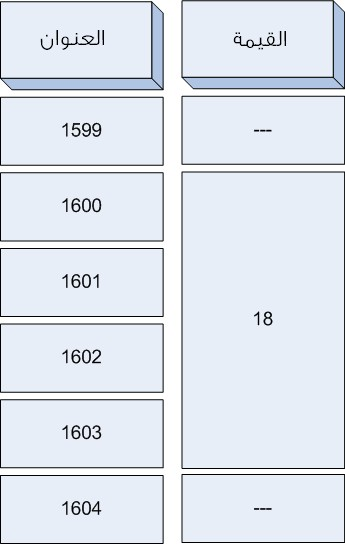
\includegraphics[width=0.3\textwidth]{Chapter_II-8_RAM-Schema-int}
\end{figure}

هنا، يمكننا فعلاً أن نرى بأن المتغير
\InlineCode{number}
من النوع
\InlineCode{int}
يحجز 4 بايت من الذاكرة.
فهو يبدأ من العنوان
$1600$
و ينتهي عند العنوان
$1603$،
المتغير القادم لن يتم تخزينه إلا إبتداءً من العنوان
$1604$ !

إن جربنا نفس الشيء مع
\InlineCode{char}،
فالمتغير لن يأخذ سوى بايت واحد في الذاكرة (الشكل التالي)~:

\begin{figure}[H]
	\centering
	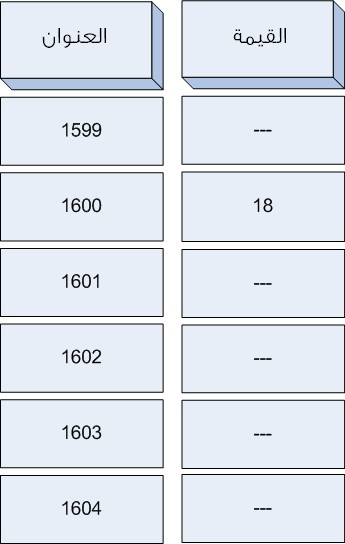
\includegraphics[width=0.3\textwidth]{Chapter_II-8_RAM-Schema-char}
\end{figure}

تخيّل الآن جدولا من
\InlineCode{int} !\\
كل "خانة" من الجدول ستحجز 4 بايت. إن كان الجدول يحوي مثلاً  100 خانة :

\begin{Csource}
int table[100];
\end{Csource}

سنحجز إذن
$100 * 4 = 400$
بايت في الذاكرة.

\begin{question}
ماذا لو كان الجدول فارغاً، هل سيحجز 400 بايت ؟
\end{question}

نعم بالطبع ! فالمكان  في الذاكرة قد تمّ حجزه، و لا يملك أي برنامج الحقّ في استخدام هذه الخانات (غير هذا البرنامج). بمجرّد التصريح عن متغيّر، سيأخذ مكانه مباشرة المكان في الذاكرة.

لاحظ لو أننا ننشئ جدولا من نوع
\InlineCode{Coordinates} :

\begin{Csource}
Coordinates table[100];
\end{Csource}

سيستخدم هذه المرّة
$8 * 100 = 800$
بايت.

من المهمّ الفهم الجيّد لهذه الحسابات البسيطة لنواصل بقيّة الفصل.

\section{الحجز الحيّ للذاكرة}

فلندخل إلى صلب الموضوع. سأذكّرك بهدفنا : تعلّم كيفيّة طلب الذاكرة يدوياً.

سنحتاج إلى تضمين المكتبة
\InlineCode{stdlib.h}.
إن كنت قد اتّبعت نصائحي، فقد ضمّنتها في كلّ برامجك. هذه المكتبة تحتوي على دالّتين سنحتاج إليهما :

\begin{itemize}
  \item \InlineCode{malloc} ("\textenglish{Memory ALLOcation}"
بمعنى "حجز الذاكرة") : تطلب الإذن من نظام التشغيل لاستخدام الذاكرة.
  \item \InlineCode{free}
(تحرير) : تسمح للإشارة لنظام التشغيل بأننا لم نعد بحاجة إلى الذاكرة الّتي طلبناها. المكان في الذاكرة تمّ تحريره، يستطيع برنامج آخر الآن استخدامها عند الحاجة.
\end{itemize}

عندما تقوم بحجز يدوي للذاكرة، فعليك اتباع الخطوات التالية :

\begin{enumerate}
  \item استدعاء
\InlineCode{malloc}
من أجل طلب الذاكرة.
  \item اختبار القيمة التي تم إرجاعها من طرف
\InlineCode{malloc}
لمعرفة ما إن نجح نظام التشغيل في حجز الذاكرة.
  \item ما إن ننتهي من استخدام الذاكرة، يجب علينا تحريرها باستعمال
\InlineCode{free}.
إن لم نفعل هذا، فسنتعرّض لتسريبات ذاكرة، أي أنّ البرنامج يخاطر بحجز كثير من الذاكرة مع أنّه ليس بحاجة إلى كلّ هذا المكان.
\end{enumerate}

هل تتذكّرك هذه الخطوات الثلاث في فصل الملفات ؟ نعم يجب أن تفعل ! المبدأ واحد تماما : نحجز، نختبر إن نجح الحجز، ثمّ نحرر عندما ننتهي من الاستعمال.

\subsection{\texttt{malloc} لنطلب الإذن لحجز الذاكرة}
نموذج الدالة
\InlineCode{malloc}
هزليّ جدّا، سترى :

\begin{Csource}
void* malloc(size_t numberOfNecessaryBytes);
\end{Csource}

الدالة تأخذ معاملا واحدا : عدد البايتات الّتي يجب حجزها. هكذا، يكفي كتابة
\InlineCode{sizeof(int)}
لحجز مكان من أجل تخزين
\InlineCode{int}.

و لكنّ الشيء الذي يثير الفضول، هو القيمة التي ترجعها الدالة : إنّها تعيد \dots
\InlineCode{void*} !
إذا لازلت تتذكّر فصل الدوال، كنت قد قلت لك بأن الكلمة
\InlineCode{void}
تعني "الفراغ" و نستعملها لنشير إلى أن الدالة لا تُعيد أية قيمة.

إذن هنا، لدينا دالة تُعيد \dots "مؤشّراً نحو فراغ" ؟ هذه نكتة جيدة !\\
يبدو أن هؤلاء المبرمجين لديهم حسّ فكاهي متطوّر.

كن متأكّدا، يوجد سبب. في الحقيقة، هذه الدالة تعيد عنوان الخانة التي حجزها نظام التشغيل من أجل متغيّرك. إن استطاع النظام إيجاد مكان لك في العنوان
$1600$،
فالدالة ستعيد مؤشّرا يحوي العنوان
$1600$.

المشكل هو أن الدالة
\InlineCode{malloc}
لا تعرف نوع المتغير التي نريد إنشاءه. في الواقع، أنت لا تعطيها سوى معامل واحد~: عدد البايتات في الذاكرة الّتي تحتاجها. فإذا طلبت 4 بايت، فهذا يمكن أن يعني
\InlineCode{int}
أو ربما
\InlineCode{long}
مثلا !

بما أنّ
\InlineCode{malloc}
لا تعرف أيّ نوع يجب عليها أن تعيد، فهي تعيد النوع
\InlineCode{void*}.
سيكون مؤشّرا نحو
\textit{أيّ نوع كان}.
يمكننا أن نقول أنّه مؤشّر جامع.

لننتقل إلى التطبيق.\\
إذا كنت أريد الاستمتاع بإنشاء متغير من نوع
\InlineCode{int}
يدويّا في الذاكرة، يجب أن أشير للـ\InlineCode{malloc}
أنني أحتاج إلى
\InlineCode{sizeof(int)}
بايت في الذاكرة.\\
أسترجع قيمة
\InlineCode{malloc}
في مؤشر على
\InlineCode{int} :

\begin{Csource}
int* allocatedMemory = NULL; // Create a pointer on int
allocatedMemory = malloc(sizeof(int)); // The function malloc puts the allocated address in the pointer.
\end{Csource}

في نهاية هذه الشفرة،
\InlineCode{allocatedMemory}
هو مؤشّر يحتوي على عنوان حجزه نظام التشغيل لك، لنقل مثلا القيمة
$1600$
للإكمال من مخططاتي السابقة.

\subsubsection{اختبار المؤشّر}
الدالة
\InlineCode{malloc}
أعادت في المتغير
\InlineCode{allocatedMemory}
عنوان الخانة التي تم حجزها بالذاكرة. هناك احتمالان :
\begin{itemize}
  \item إذا نجح الحجز، فالمؤشّر سيحتوي عنوانا.
  \item إذا فشل الحجز، فالمؤشّر سيحتوي العنوان
\InlineCode{NULL}.
\end{itemize}

إنه من النادر أن تفشل عملية حجز الذاكرة، لكن هذا ممكن. تخيّل أنك تطلب حجز
\textenglish{34 Go}
من الذاكرة العشوائية، في هذه الحالة، ستفشل عملية الحجز على أغلب الظن.

من المستحسن دائماً أن نختبر ما إن تمت العملية بنجاح. سنفعل هذا : إن فشل الحجز، فهذا يعني أن المساحة الحرّة من الذاكرة العشوائية لم تكن كافية (هذه حالة حرجة). في حالة كهذه، يجب إيقاف البرنامج فورا لأنّه، على أية حال، لن يكون قادراً على الاستمرار بشكل عاديّ.

سنستعمل دالة قياسيّة لم يسبق لنا رؤيتها حتّى الآن :
\InlineCode{exit()}.
هذه الأخيرة توقف البرنامج فورا. إنّها تأخذ معاملا : القيمة الّتي يجب إعادتها من طرف البرنامج (هذا في الحقيقة يوافق الـ\InlineCode{return}
الخاص بالـ\InlineCode{main}).

\begin{Csource}
int main(int argc, char *argv[])
{
	int* allocatedMemory = NULL;
	allocatedMemory = malloc(sizeof(int));
	if (allocatedMemory == NULL) // If the allocation has failed
	{
    	exit(0); // Stop the program
	}
	// Else, we can continue the program normally.
	return 0;
}
\end{Csource}

إذا كان المؤشر مختلفا عن
\InlineCode{NULL}،
يمكن للبرنامج أن يواصل العمل، و إلا فيجب إظهار رسالة خطأ أو حتّى إنهاء البرنامج لأنّه لن يتمكّن من الاستمرار بشكل صحيح إن لّم يكن هناك مكان في الذاكرة.

\subsection{\texttt{free} : تحرير الذاكرة}

مثلما استعملنا الدالة
\InlineCode{fclose}
لنغلق ملفاً لم نعد في حاجة إليه، سنستعمل الدالة
\InlineCode{free}
من أجل تحرير الذاكرة التي لم نعد بحاجة إليها.

\begin{Csource}
void free(void* pointer);
\end{Csource}

الدالة
\InlineCode{free}
بحاجة فقط إلى عنوان الذاكرة المراد تحريرها. سنرسل لها إذن مؤشّرنا، أي
\InlineCode{allocatedMemory}
في مثالنا.\\
إليكم المخطط الكامل و النهائي، مشابه بشكل كبير لما رأينا في الفصل الخاص بالملفات :

\begin{Csource}
int main(int argc, char *argv[])
{
	int* allocatedMemory = NULL;
	allocatedMemory = malloc(sizeof(int));
	if (allocatedMemory == NULL) // Verify if the memory has been allocated
	{
		exit(0); // Error: Stop everything !
	}
	// We can use the memory here
	free(allocatedMemory); // No need for the memory anymore, free it.
	return 0;
}
\end{Csource}

\subsubsection{مثال استخدام واقعي}

سنبرمج شيئا درسناه منذ زمن طويل : الطلب من المستخدم تزويدنا بعُمره ثمّ عرضه له. الشيء المختلف عمّا كنّا نفعله سابقا هو أن المتغيّر هنا سيتمّ حجزه يدويا (نقول أيضا حيويّا) و ليس تلقائيّا كالسابق. إذن نعم، في المرّة الأولى، الشفرة أصعب قليلا. لكن قم بالمجهود اللازم لفهمها جيّدا، هذا ضروريّ :

\begin{Csource}
int main(int argc, char *argv[])
{
	int* allocatedMemory = NULL;
	allocatedMemory = malloc(sizeof(int)); // Allocation of the memory
	if (allocatedMemory == NULL)
	{
		exit(0);
	}
	// Using the memory
	printf("How old are you ? ");
	scanf("%d", allocatedMemory);
	printf("You are %d years old\n", *allocatedMemory);
	free(allocatedMemory); // Freeing the memory
	 return 0;
}
\end{Csource}

\begin{Console}
How old are you  ? 31
You are 31 years old
\end{Console}

\begin{warning}
حذار : بما أن
\InlineCode{allocatedMemory}
هو مؤشّر، فلا نستعمله بنفس الطريقة التي نستعمل بها متغيّرا حقيقيّا. للحصول على قيمة المتغير يجب وضع نجمة أمامه :
\InlineCode{*allocatedMemory}
(لاحظ
\InlineCode{printf}).
بينما للحصول على العنوان، يكفي فقط أن كتابة اسم المؤشّر
\InlineCode{allocatedMemory}
(لاحظ
\InlineCode{scanf}).\\
كلّ هذا تم شرحه في فصل المؤشّرات. رغم ذلك، أعرف أن هذا سيأخذ وقتا و من الممكن أن تخلط بينهما. إن كانت هذه حالتك، فعليك بإعادة قراءة فصل المؤشّرات، فهو أساسي.
\end{warning}

لنعد إلى الشفرة. لقد قمنا بحجز حيّ لمتغيّر من نوع
\InlineCode{int}.
في النهاية، ما كتبناه يعود تماما لاستخدام الطريقة
"التلقائيّة" الّتي نعرفها الآن جيّدا :

\begin{Csource}
int main(int argc, char *argv[])
{
	int myVariable = 0; // Allocation of the memory (automatically)
	// Using the memory
	printf("How old are you ? ");
	scanf("%d", &myVariable);
	printf("You are %d years old\n", myVariable);
	return 0;
} // Freeing the memory (automatically at the end of the function)
\end{Csource}

\begin{Console}
How old are you ? 31
You are 31 years old
\end{Console}

كملخص، لدينا طريقتان لإنشاء متغير، أي لحجز الذاكرة. إمّا أن نقوم بذلك :
\begin{itemize}
  \item تلقائيّا : هي الطريقة الّتي تعرفها و التي استعملناها لغاية الآن.
  \item يدويا (حيويّا) : هي الطريقة الّتي أعلّمك إيّاها في هذا الفصل.
\end{itemize}

\begin{question}
أنا أجد أن الطريقة الحيّة معقّدة و بلا فائدة !
\end{question}

أكثر تعقيدا \dots بالتأكيد. لكن بدون فائدة، لا ! أحيانا نكون مجبرين على حجز الذاكرة يدويّا كما سنرى الآن.

\section{الحجز الحيّ لجدول}
لحد الآن استعملنا الحجز الحي لإنشاء متغيّر صغير. عادة لا نستخدم الحجز الحيّ في هذا. نستخدم الطريقة التلقائيّة الّتي هي أبسط.

متى نحتاج للحجز الحيّ، تتسائلون ؟ أكثر شيء، نستخدمه لإنشاء جدول لا نعرف حجمه قبل تشغيل البرنامج.

لنتخيل مثلا برنامجاً يقوم بتخزين أعمار أصدقاء المستخدم في جدول، يمكنك فعل ذلك هكذا :

\begin{Csource}
int friendsAge[15];
\end{Csource}

لكن من قال أنه لديه 15 صديقا ؟ ربما لديه أكثر من هذا !
عندما تكتب الشفرة المصدريّة، لا يمكنك معرفة حجم الجدول قبل التشغيل، عندما تطلب من المستعمل إدخال عدد الأصدقاء.

فائدة الحجز الحيّ موجودة هنا : تطلب من المستخدم إدخال عدد الأصدقاء، ثم تنشئ جدولا لديه تماما الحجم اللازم (لا أصغر و لا أكبر). إن كان للمستخدم 15 صديقا، فسننشئ جدولا من 15
\InlineCode{int}،
إن كان لديه 28، فسننشئ جدولا من 28
\InlineCode{int}،
إلخ.

كما علّمتك، من الممنوع في لغة الـ\textenglish{C}
إنشاء جدول بتحديد حجمه باستخدام متغيّر :

\begin{Csource}
int friends[friendsNumber];
\end{Csource}

\begin{information}
هذه الشفرة قد تعمل في بعض المترجمات لكن في حالات معيّنة، من المنصوح به عدم استخدامها~!
\end{information}

فائدة الحجز الحيّ، هي أنّه يمكننا من إنشاء جدول حجمه تماما المتغيّر
\InlineCode{friendsNumber}.
و هذا بفضل شفرة تعمل في كلّ مكان !

سنطلب من
\InlineCode{malloc}
حجز
\InlineCode{friendsNumber * sizeof(int)}
بايت في الذاكرة :

\begin{Csource}
friends = malloc(friendsNumber * sizeof(int));
\end{Csource}

هذه الشفرة تسمح بإنشاء جدول من نوع
\InlineCode{int}
حجمه بوافق تماما عدد الأصدقاء !

هذا ما يقوم به البرنامج بالترتيب :

\begin{enumerate}
  \item نطلب من المستخدم كم من صديق لديه.
  \item إنشاء جدول من
\InlineCode{int}
ذو حجم يساوي عدد أصدقائه (باستخدام
\InlineCode{malloc}).
  \item نطلب كم عمر كلّ واحد من أصدقائه واحدا واحدا، و نقوم بتخزينها في الجدول.
  \item نظهر أعمار الأصدقاء من محتوى الجدول لنتأكد بأننا خزّننا كلّ شيء.
  \item في النهاية، و بما أننا لسنا بحاجة إلى الجدول الذي يحوي أعمار الأصدقاء، نقوم بتحريره بالدالة
\InlineCode{free}.
\end{enumerate}

\begin{Csource}
int main(int argc, char *argv[])
{
  int friendsNumber = 0, i = 0;
  int* friendsAge = NULL; // We use it after calling malloc
  // Request for friends count
  printf("How many friends do you have ? ");
  scanf("%d", &friendsNumber);
  if (friendsNumber > 0) // The user must have at least one friend (or i will be upset :p)
  {
    friendsAge = malloc(friendsNumber * sizeof(int)); // Allocate the memory for the table
    if (friendsAge == NULL) // Verify the allocation
    {
      exit(0); // Stop everything
    }
    // Request for the ages one by one
    for (i = 0 ; i < friendsNumber ; i++)
    {
      printf("How old is the friend number %d ? ", i + 1);
      scanf("%d", &friendsAge[i]);
    }
    // Display the stored ages
    printf("\n\nYour friends have the next ages :\n");
    for (i = 0 ; i < friendsNumber ; i++)
    {
      printf("%d years\n", friendsAge[i]);
    }
    // Free the memory
    free(friendsAge);
  }
  return 0;
}
\end{Csource}

\begin{Console}
How many friends do you have ? 5
How old is the friend number 1 ? 16
How old is the friend number 2 ? 18
How old is the friend number 3 ? 20
How old is the friend number 4 ? 26
How old is the friend number 5 ? 27
Your friends have the next ages :
16 years
18 years
20 years
26 years
27 years
\end{Console}

هذا البرنامج عديم الفائدة : يطلب الأعمار ثمّ يعرضها بعد ذلك. لقد اخترت فعل هذا لأنّه مثال "بسيط" (هذا إن فهمت
\InlineCode{malloc}).

أؤكّد لك : في بقيّة هذا الكتاب ستكون لنا فرص لاستخدام
\InlineCode{malloc}
في أمور أكثر إفادة من تخزين أعمار الأصدقاء !

\section*{ملخّص}

\begin{itemize}
  \item كل متغير يحجز مكانا مختلفا في الذاكرة و هذا حسب نوعه.
  \item يمكننا معرفة عدد البايتات التي يشغلها كل نوع باستعمال العامل \InlineCode{sizeof()}.
  \item الحجز الحيّ هو عبارة عن حجز يدوي لمكان في الذاكرة من أجل متغير أو من جدول.
  \item الحجز الحيّ يتم باستعمال الدالة
\InlineCode{malloc()}
و يجب خاصّة عدم نسيان تحرير الذاكرة باستعمال
\InlineCode{free()}
بمجرّد الانتهاء من الاستخدام.
  \item الحجز الحيّ يسمح بشكل أساسيّ بتعريف جدول حجمه يتمّ تعيينه بمتغيّر في حين تشغيل البرنامج.
\end{itemize}
